\documentclass[chi_draft]{sigchi}

% Use this section to set the ACM copyright statement (e.g. for
% preprints).  Consult the conference website for the camera-ready
% copyright statement.

% Copyright
\CopyrightYear{2017}
%\setcopyright{acmcopyright}
\setcopyright{acmlicensed}
%\setcopyright{rightsretained}
%\setcopyright{usgov}
%\setcopyright{usgovmixed}
%\setcopyright{cagov}
%\setcopyright{cagovmixed}
% DOI
\doi{http://dx.doi.org/10.475/123_4}
% ISBN
\isbn{123-4567-24-567/08/06}
%Conference
\conferenceinfo{IoT}{...}
%Price
\acmPrice{\$15.00}

% Use this command to override the default ACM copyright statement
% (e.g. for preprints).  Consult the conference website for the
% camera-ready copyright statement.

%% HOW TO OVERRIDE THE DEFAULT COPYRIGHT STRIP --
%% Please note you need to make sure the copy for your specific
%% license is used here!
% \toappear{
% Permission to make digital or hard copies of all or part of this work
% for personal or classroom use is granted without fee provided that
% copies are not made or distributed for profit or commercial advantage
% and that copies bear this notice and the full citation on the first
% page. Copyrights for components of this work owned by others than ACM
% must be honored. Abstracting with credit is permitted. To copy
% otherwise, or republish, to post on servers or to redistribute to
% lists, requires prior specific permission and/or a fee. Request
% permissions from \href{mailto:Permissions@acm.org}{Permissions@acm.org}. \\
% \emph{CHI '16},  May 07--12, 2016, San Jose, CA, USA \\
% ACM xxx-x-xxxx-xxxx-x/xx/xx\ldots \$15.00 \\
% DOI: \url{http://dx.doi.org/xx.xxxx/xxxxxxx.xxxxxxx}
% }

% Arabic page numbers for submission.  Remove this line to eliminate
% page numbers for the camera ready copy
% \pagenumbering{arabic}



%% PM Define authornote command for comments
\newcommand{\authornote}[1] {
    \begin{center}
        \framebox{
            {\begin{minipage}[t]{0.9\linewidth}
                \raggedright  \textbf{[PM]}~ \scriptsize #1 \normalsize
            \end{minipage}}
    }
    \end{center}
}

\usepackage{color}
\definecolor{highlight}{rgb}{1,1,0.6}
\definecolor{link}{rgb}{0.5,0.0,0.0}
\definecolor{cite}{rgb}{0.0,0.0,0.6}
\definecolor{url} {rgb}{0.3,0.0,0.3}
\definecolor{grey}{rgb}{0.3,0.3,0.3}


\usepackage[pdftex]{hyperref}
\hypersetup{%
	%pdftitle={\myTitle}, %
	pdfauthor={blind submission}, %
	%pdfkeywords={\programname},%
	bookmarksnumbered, %
	pdfstartview={c}, %
	colorlinks,%
	citecolor=black, %
	filecolor=black, %
	linkcolor=black, %
	urlcolor=black}

\usepackage{soul}
% % annotations environments % % 
\newcommand{\note}[1]{\textit{\textcolor{red}{\{#1\}}}}
\sethlcolor{highlight}

\newcommand{\comment}[2]{\hl{#1} {\color{red}\textit{\{#2\}}}}




\begin{document}
%
% paper title
% Titles are generally capitalized except for words such as a, an, and, as,
% at, but, by, for, in, nor, of, on, or, the, to and up, which are usually
% not capitalized unless they are the first or last word of the title.
% Linebreaks \\ can be used within to get better formatting as desired.
% Do not put math or special symbols in the title.
\title{Mind My Value: a decentralized infrastructure for fair and trusted IoT data trading}


%\title{\plaintitle}

\numberofauthors{5}
\emptyauthor
%\author{%
%	\alignauthor{Paolo Missier\\
%		\affaddr{Newcastle University}\\
%		\affaddr{Newcastle, UK}\\
%		\email{paolo.missier@newcastle.ac.uk}}\\
%	\alignauthor{Michele Nati\\
%		\affaddr{Digital Catapult}\\
%		\affaddr{London, UK}\\
%		\email{michele.nati@digicatapult.org.uk}}\\
%	\alignauthor{Angelo Capossele\\
%		\affaddr{Digital Catapult}\\
%		\affaddr{London, UK}\\
%		\email{Angelo.Capossele@digicatapult.org.uk}}\\
%	\alignauthor{Andrea Gaglione\\
%	\affaddr{Digital Catapult}\\
%	\affaddr{London, UK}\\
%	\email{Andrea.Gaglione@digicatapult.org.uk}}\\
%	\alignauthor{Shaimaa Bajoudah\\
%	\affaddr{Newcastle University}\\
%	\affaddr{Newcastle, UK}\\
%	\email{S.Bajoudah1@newcastle.ac.uk}}\\
%}


% make the title area
\maketitle

% As a general rule, do not put math, special symbols or citations
% in the abstract
\begin{abstract}
Internet of Things data are increasingly viewed as a new form of massively distributed and large scale digital assets, which are continuously generated by millions of connected devices.
The real value of such assets can only be realised by allowing IoT data trading to occur on a marketplace that rewards every single producer and consumer, at a very granular level.
Crucially, we believe that such a marketplace should not be owned by anybody, and should instead fairly and transparently self-enforce a well defined set of governance rules.
In this paper we address some of the technical challenges involved in realising such a marketplace.
We leverage emerging blockchain technologies to build a decentralised, trusted, transparent and open architecture for IoT traffic metering and contract compliance, on top of the largely adopted IoT brokered data infrastructure.
We discuss an Ethereum-based prototype implementation and experimentally evaluate the overhead cost associated with Smart Contract transactions, concluding that a viable business model can indeed be associated with our technical approach.
\end{abstract}

\section{Introduction}
Much of the expected value associated with the growing industry of Internet of Thing devices \cite{7004800} is to be found in the streams of data generated by those devices.
Application areas where interest in IoT data streams is growing range from health care \cite{7113786} to personal fitness, smart cities \cite{Perera2014}, optimisation of energy consumption in the home, and many more.
In each of these areas, the value of IoT is only delivered when the continuous data streams produced at the edge of the network are aggregated and analysed, either individually or as ``big data'' aggregations over time and over segments of the population.  We refer to these consumers as Value Added Services (VAS).

Some of these applications are just emerging.
For example, in a public transport network like the London underground, the density of personal travel card swipes over time at individual metro stations may be
useful not only to the transportation authority, but also to taxi companies, which can benefit from the knowledge of any anomalous passenger traffic pattern, i.e., by placing their fleet at the right stations at the right time. A VAS that specialises in data analytics may therefore buy metro passenger data together with footfall data collected, for example, through an IoT infrastructure, and sell
recommendation services to taxi companies.

In response to this ``technology push'', new business models are indeed emerging \cite{Stahl2016,7765669} where data are viewed as tradeable digital assets. 
In this paper we propose an initial technical infrastructure for a new kind of data marketplace that, in the long run, is designed to meet four main requirements.
First, the marketplace should be dynamic and flexible in order to enable the new and un-anticipated kind of business relationships just illustrated. It should be possible to quickly  establish and then fulfil contracts between one and possibly many producers and the VAS, with guarantees of compliance and fairness.

Second, the marketplace should allow not only organisations, but also individuals to offer their data. 
%
For example, today it is possible to quantify an athlete's effort during a competition using a number of wearable devices, from bio-harness to accelerometers, to video feeds.
One can imagine that individuals may decide to let VAS access their data feeds, in return for some benefit (monetary or otherwise).
In the near future, athletes may be able to sell these feeds to followers who are interested in tracking their competition online.
There are examples in the UK today, where individuals get heavy discounts on smart watches from health insurance companies, provided they let the company access their fitness data.

Third, the main asset traded in the marketplace are streams of IoT data. This is not usual: a 2012 survey of data vendors \cite{Schomm2013}, for example, includes 46 data suppliers, however the definition of data marketplace used in the paper is generic (``a platform on which anybody can upload and maintain data sets, with license-regulated access to and use of the data'') and geared towards static data, like Microsoft's Azure Data Market.
In contrast, our requirement entails the typical ``Big Data'' challenges of high Volume, high Velocity, and high Variety of the streams.

Finally, it should be possible to run a completely decentralised marketplace which operates according to governance rules, which determine what kinds of contract and transactions are acceptable, and stipulate sanctions when the rules are violated. 
However, contrary to current proposals, eg \cite{Cao:2016:MMR:2926746.2883611}, we are going to assume  there is no central trusted authority appointed to enforce those rules. The assumption is that due to the unpredictable variety of actors involved in such a marketplace, a multi-stakeholders decentralised trust will better adapt than a centralised one.
In the paper we focus specifically on this novel aspect. We investigate the use of blockchain (distributed ledger), and specifically of Smart Contracts \cite{Buterin2014}, as a technology enabler for an authority-free, trusted data merketplace.

In summary, we envision a decentralised, self-regulating IoT data marketplace where governance rules are automatically enforced and fairness of the transactions is regulated by means of a trust model amongst participants.

The contributions in the paper can be summarised as following.
%
First,  we present a conceptual model for tracking brokered IoT data flows from gateways to VAS in the cloud, which embodies a methodology to achieve granular metering of IoT data exchanges.

Second, we explore the use of blockchain technology and Smart Contracts to remove the need for a centralised trust when settling contracts. 

Third, we present a proof-of-concept implementation of this marketplace enabling infrastructure. For this, we have adapted the popular open source Mosquitto MQTT broker to add traffic metering capabilities, and use the Ethereum smart contracts technology for enforcing contract definition and trigger dispute resolution.

Finally, we carry out an experimental evaluation where we identify the viable boundaries for the prices of digital assets, which make the marketplace economically sustainable relative to the number and frequency of transactions, taking account of the current Ethereum Smart Contract cost model.
We assess the capability of Ethereum Smart Contracts to handle a stream of contract settlements at varying arrival rate, and conclude that they are indeed a viable option for the validation of contract compliance.
As the use of Smart Contracts is a novel feature for any IoT architecture, we conclude the paper with a discussion on the challenges and lesson learnt from the use of this emerging and enabling technology.

%In the health sector, for example, individuals' activity levels and fitness data, as recorded by smart phones or dedicated fitness devices, may be of interest to health care providers as well as health insurance companies, even if only in anonymised and aggregate form.
%
%
%While we acknowledge that contractual agreements must be stipulated between %the 
%individuals or organisations that own or control the devices and the VASs, in this work we %are only concerned with the study of 
%focus on the underpinning technology that %makes it possible to realise 
%enable IoT data trading by enhancing the current IoT infrastructure%regardless of specific pricing and contract models.,
%, and analyse its feasibility by quantifying the actual value of both data and transactions. 

%The main novel element of our work is that we challenge the common assumption that a marketplace must be controlled by a trusted authority, in charge of certifying the identity of the participants%, 
% and ensuring %fairness.
%fair value distribution. 
%In particular, data brokers typically play the role of trusted network components that are controlled by a marketplace authority.
%%
%

%\note{\cite{7004800} Perera, C., Liu, C. H.,\& Jayawardena, S. (2015). The Emerging Internet of Things Marketplace From an Industrial Perspective: A Survey. IEEE Transactions on Emerging Topics in Computing, 3(4), 585–598. https://doi.org/10.1109/TETC.2015.2390034\\
%	A comprehensive survey of industry-ready IoT technology -- good to support the claim that there are a lot of sensor types out there, but ``marketplace''  here just means, HW that is on the market...}

%In the rest of the paper we present our approach to addressing some of the challenges that emerge when trying to realise such a trust-less IoT data marketplace.

%Our first contribution is a data architecture for tracking data flows through brokers, using a publish-subscribe pattern, or through network servers, to achieve granular metering of IoT data exchanges.

%Secondly, we explore the use of blockchain technology and \textit{Smart Contracts} \cite{SMART-CONTRACTS} to remove the need for centralised trust. We discuss the challenges and limitations of using Smart Contracts for automatic dispute resolution.

%Finally, we present a prototype realisation of the marketplace, using MQTT brokers for granular data exchange with added traffic metering capabilities, and the Ethereum Smart Contracts technology for enforcing the contracts definition and providing dispute resolution capabilities.

%In our initial evaluation we show that smart contracts are indeed a viable option for validation of contract compliance, and assess its capability to handle a stream of blockchain transactions at varying arrival rate.


\subsection{Background and Related work}

%%%%
% sensors as service
%%%%
%\note{   \cite{Perera2014}  Perera, C., Zaslavsky, A., Christen, P., \& Georgakopoulos, D. (2014). Sensing as a service model for smart cities supported by Internet of Things. Transactions on Emerging Telecommunications Technologies, 25(1), 81–93. https://doi.org/10.1002/ett.2704}

%\note{ \cite{distefano2012sensing}  Distefano, S., Merlino, G., \& Puliafito, A. (2012). Sensing and actuation as a service: A new development for clouds. In Network Computing and Applications (NCA), 2012 11th IEEE International Symposium on (pp. 272–275). }

%\note{Banerjee, P., Friedrich, R., Bash, C., Goldsack, P., Huberman, B., Manley, J., … Veitch, A. (2011). Everything as a Service: Powering the New Information Economy. Computer, 44(3), 36–43. https://doi.org/10.1109/MC.2011.67}

The idea of considering data from IoT sensors as tradeable assets is closely related to that of \textit{Sensing as a Service} (SaaS) models, or even \textit{Sensing and Actuation as a service} (SAaaS) \cite{distefano2012sensing}, themselves derivatives of the more general ``Everything as a Service'' (XAAS) cloud-based model for data exchange \cite{5719575}. Perera et al. \cite{Perera2014}, for instance, outline a vision of a near future for Smart Cities, where data streams emanating from pervasive Internet of Things sensors are accessible through services. The SaaS model consists of four conceptual layers: sensors and their owners, sensor publishers, service providers, and sensor data consumers. In this classification, our work is relevant to all of these agents, as it enables fair and metered data exchanges amongst sensors owners and publishers on one side, and sensor data consumers, on the other.


%%%%
%\note{related: data pricing}
%%%%
%\note{\cite{Li:2014:TPP:2691190.2691191} Li, C., Li, D. Y., Miklau, G., \& Suciu, D. (2014). A Theory of Pricing Private Data. ACM Trans. Database Syst., 39(4), 34:1--34:28. https://doi.org/10.1145/2691190.2691191}

%\note{\cite{7437020} Niyato, D., Hoang, D. T., Luong, N. C., Wang, P., Kim, D. I., \& Han, Z. (2016). Smart data pricing models for the internet of things: a bundling strategy approach. IEEE Network, 30(2), 18–25. https://doi.org/10.1109/MNET.2016.7437020}

%\note{related: trust management}
%\note{ \cite{Bao:2012:DTM:2378023.2378025} Bao, F., \& Chen, I.-R. (2012). Dynamic Trust Management for Internet of Things Applications. In Proceedings of the 2012 International Workshop on Self-aware Internet of Things (pp. 1–6). New York, NY, USA: ACM. https://doi.org/10.1145/2378023.2378025}

%\note{\cite{Yan2014a} Yan, Z., Zhang, P., \& Vasilakos, A. V. (2014). A survey on trust management for Internet of Things. Journal of Network and Computer Applications, 42, 120–134. https://doi.org/10.1016/j.jnca.2014.01.014}
%

Our traffic monitoring infrastructure assumes that suitable pricing models that associate values to messages are in place.
However, it is agnostic and ``orthogonal'' to the specific pricing model, as long as the price of a complex bundle of data offering can be expressed in terms of unit cost associated to individual messages. 
Thus, in principle, any of the existing models for data pricing may be used in combination with traffic metering. Such models, recently proposed, range from theoretical frameworks for assigning prices to query answers as a function of their accuracy \cite{Li:2014:TPP:2691190.2691191}, to adaptations of \textit{Smart Data Pricing} \cite{Sen:2015:SDP:2847579.2756543} to the dynamic pricing of IoT data, such as personal data from wearable sensors \cite{7437020}.

A trust management model should also be established, i.e., to enable self-regulation of marketplace rules as we briefly discuss at the end of the paper.
Again, while this is out of our scope, existing frameworks can be used on top of our infrastructure.
Yan et al \cite{Yan2014a} provide a starting point, by exploring the notion of trust across the IoT platform layers (physical sensing, network, and application layer), with focus on  a wide range of properties from security to goodness, strength, reliability, availability, ability of data. Interestingly, however, their survey largely overlooks issues of trust amongst participants in a data marketplace, i.e., in the context of data exchange transactions.

%\note{ Roman, D., \& Stefano, G. (2016). Towards a Reference Architecture for Trusted Data Marketplaces: The Credit Scoring Perspective. In 2016 2nd International Conference on Open and Big Data (OBD) (pp. 95–101). IEEE. https://doi.org/10.1109/OBD.2016.21}
More directly useful in our setting, as we progress in our work, is Roman and Gatti's study of trust in data marketplaces \cite{7573695}, based on \textit{credit scoring}, where a direct connection is made to the use of blockchain technology in connection with data trading.

%%%%
%\note{related: marketplace for data}
%%%%

Two technical architectures for data marketplaces are directly relevant to our work.
%\note{ Schomm, F., Stahl, F., \& Vossen, G. (2013). Marketplaces for Data: An Initial Survey. SIGMOD Rec., 42(1), 15–26. https://doi.org/10.1145/2481528.2481532}
%\note{\cite{Cao:2016:MMR:2926746.2883611}  Cao, T.-D., Pham, T.-V., Vu, Q.-H., Truong, H.-L., Le, D.-H., \& Dustdar, S. (2016). MARSA: A Marketplace for Realtime Human Sensing Data. ACM Trans. Internet Technol., 16(3), 16:1--16:21. https://doi.org/10.1145/2883611}
Firstly the MARSA platform \cite{Cao:2016:MMR:2926746.2883611}, designed specifically to deal with real-time data streams by interacting with existing IoT platforms.
The motivation for this work is very similar to ours, namely to provide a marketplace where owners have an incentive to trade their data, for either personal or community benefit.
The many technical requirements that emerge from analysis of data marketplace potential translate into a complex architecture, which includes data flow orchestration, participants registration, data contract management, and payment.  
While these components do address complex marketplace requirements, our main challenge, namely to remove the need for a central trusted authority to manage the marketplace and ensure its fairness, remains unique to our work.

Secondly, Misura, K., \& Zagar \cite{7765669} focus on a query-based mechanism, whereby devices register their data supply capabilities to a broker along with a number of properties, and consumers express interest in data streams by querying those properties. The broker then connects the supplier stream to the consumer, and monitors usage. 
This is relevant work, as this type of matching of consumer data requirements to suppliers capabilities is more sophisticated than simple topic subscription. Our work is complementary to this  and also contributes to remove the trust from the broker for monitoring usage.
In our future work. we plan to move away from a fine-grained data subscription and towards complex data contracts (bundles), as discussed briefly at the end of the paper.
%\note{ Misura, K., \& Zagar, M. (2016). Data marketplace for Internet of Things. In 2016 International Conference on Smart Systems and Technologies (SST) (pp. 255–260). IEEE. https://doi.org/10.1109/SST.2016.7765669}
%\note{\cite{7146004} Blazquez, A., Tsiatsis, V., \& Vandikas, K. (2015). Performance Evaluation of OpenID Connect for an IoT Information Marketplace. In 2015 IEEE 81st Vehicular Technology Conference (VTC Spring) (pp. 1–6). IEEE. https://doi.org/10.1109/VTCSpring.2015.7146004}	

\section{Brokered IoT data as tradeable assets}

We now present our conceptual model for the specification and enforcement of streamed data exchange agreements.
%
Following common IoT infrastructures, we are going to assume that data exchanges are mediated by one or more brokers.
Initially we assume the brokers are trusted. In Sec. \ref{sec:no-trust} we are going to explore the consequences of relaxing this assumption.

\subsection{Contracts and pricing}

Let  $P = \{p_1 \dots p_n \}$ and $C = \{ c_1 \dots c_m \}$ denote the set of producers (IoT devices) and consumers (VAS) that participate in the marketplace, respectively.
%
In the standard publish/subscribe model for data brokering, the $p_i$ act as publishers and the $c_j$ are subscribers.
These participants agree on a set $T = \{ t_1 \dots t_r \}$ of topics.
In IoT data brokering, messages are generated by gateways, which are responsible for segmenting raw data streams from edge devices into discrete messages.
The topic associated with each message describes the type of data stream, for example ``heart rate'', ``GPS track'', ``glucose reading'', ``energy reading'', etc.

Suppose $ p_i $ publishes data on a set of topics $T_{i} \subset T$.
A consumer $ c_j  $ enters into a \textit{contractual agreements} with a producer $ p_i  $ by subscribing to a subset $T_{ij} \subset T_i$ of the topics available from $p_i$, possibly only for the duration of a time window $ W = [w_s, w_e] $.
Such an agreement is interpreted as ``$p_i$ agrees to let $c_j$ receive a copy of all its messages tagged with any $t \in T_{ij}$ during $W$, and $c_j$ agrees to pay a corresponding data exchange fee. 
The broker manages all subscriptions and is responsible for reliably delivering to $ c_j  $ a copy of each message that has a topic that $ c_j $ subscribes to.

Note that in the standard pub/sub model, publishers and subscribers are unaware of one another, and their interaction is entirely mediated by the broker. 
However, it is easy to to extend the model by assuming that the broker will only deliver messages from $ p_i $ to $ c_j $ if $ c_j $ has an active agreement (i.e., relative to $W$) with $ p_i $.\footnote{This can be easily realised in a MQTT-based broker, which we use in our reference implementation, e.g., by encrypting payload data}

%for instance by embedding a device name into a topic tree
%	
%	. When topics are into a hierarchy, 
%
%\textcolor{blue}{To enable explicit marketplace} interactions, we propose a variation of the model whereby every message topic embeds the publisher's ID, which in combination with MQTT's topic regular expressions capability enables a subscriber to selectively choose the stream they intend to license.
%For example, device ``1234'' may publish messages about a specific room's temperature using topic  \#/temperature/1234/living\_room\_temperature. 
%A subscriber may choose to subscribe to this specific topic, or to any  living\_room\_temperature message using expression \#/temperature/*/living\_room\_temperature, or to any generic temperature message from ``1234'' or from any publisher.

%Note incidentally that the model includes the case, not shown in the figure, where a VAS may aggregate data from multiple $ p_i $s and then publish this value-added data, enabling other VAS to license it. 
%In this case, a VAS is both a consumer and a producer.



%While a variety of pricing models have recently been proposed for digital assets in emerging data marketplace scenarios \note{CITE}, discussing how the marketplace sets the data prices is beyond the scope of this work. Instead, we are simply going to assume that each individual message is a digital asset with a constant unit value $\mathit{val}(t_k)$, which is determined solely by the message's topic $t_k$.
A variety of pricing models have recently been proposed for digital assets in emerging data marketplace scenario \cite{Sen:2015:SDP:2847579.2756543,Li:2014:TPP:2691190.2691191,7553037,7437020}.
In this work we are going to assume a simple model where each individual message has constant unit value $\mathit{val}(t_k)$, which is determined solely by the message's topic $t_k$. 
While our infrastructure is largely agnostic to the specific data pricing model, in our evaluation we analyse the economic sustainability of a decentralised marketplace. Specifically, in Sec.\ref{sec:evaluation} we analyse the cost overhead of enforcing agreements given the current cost model associated with Smart Contract transactions.

\subsection{Data traffic cubes and centralised settlement}

Contract enforcement and settlement involves calculating the total price associated with the messages that have been routed from each $ p_i $ to each $ c_j $ within each $W$.
Since we have assumed that the price is  determined only by the number of messages and the unit cost for each topic, this simply requires keeping a count of the number of messages about topic $t_k$ that originated from $p_i$ and reached $c_j$ during $W$, grouped by $ p_i $, $ c_j $, and $ t_k $.
We denote each of these counts as $N_{ijk}(W)$.

Generating these counts requires that the broker be capable of \textit{metering} all traffic, that is, of logging all messages.
The log consists of a set of tuples:
$ \{\langle p_i, c_j, t_k \rangle  \} $

At the end of each $W$, the log is aggregated over each $p_i \in P, c_j \in C, t_k \in T$, resulting in a set of tuples that we call a \textit{traffic cube}:
\begin{equation}\label{eq:cube}
\mathit{cube}(W) = \{ \langle p_i, c_j, t_k, N_{ijk}(W) \rangle \}_{p_i \in P, c_j \in C, t_k \in T}
\end{equation}

Here we borrow our terminology from standard database practice (OLAP, or Online Analytical data Processing), where a  ``cube'' is a table with $ N $ attributes, in which the first $ N-1 $ attributes are  dimensions in a database schema (in our case, these are the Producers, Consumers (the VAS), and Topics) and the last is an aggregation over values in the database for each combination of the dimensions -- in our case, a count().
We use a matrix indexing notation to refer to specific cells in the cube, i.e.:
\[ \mathit{cube}(W)[p_i, c_j, t_k] = N_{ijk}(W) \] 
These cubes contain summaries of all data flows observed by a broker. Notice that they only contain \textit{metadata}, i.e., the counts, but not the content of the messages.
%
Note that the values in the cube may be sparse, i.e., $N_{ijk}(W) = 0$ whenever $c_j$ does not subscribe to $t_k$.

\textit{Settlement} is the process of calculating the total fee owed by each $ c_j $ to each $ p_i $ at the end of each $W$.
This is computed by suitably aggregating the counts in the cube, namely:
\begin{equation}
\mathit{fee}(c_j, p_i, W) = \sum_{t_k \in T} N_{ijk}(W) \cdot \mathit{val}(t_k)
\label{eq:balance}
\end{equation}
and the total profit for $ p_i  $ during $W$ is
\begin{equation}
\mathit{profit}(p_i, W) = \sum_{c_j} \mathit{fee}(c_j, p_i, W)
\label{eq:reward}
\end{equation}
In the centralised scenario we have considered so far settlement is straightforward, as the broker is entrusted with generating accurate logging and thus complete and correct cubes.
Note that, under the same trust assumptions, settlement extends easily to a more realistic scenario where multiple brokers are deployed, each enhanced with the same logging capabilities and local traffic reporting service.

Hovever, settlement becomes challenging in an extended model where there is no assumption of trust in the broker.
In this case, fee settlement must rely on data traffic counts that are calculated independently by each participant, based on the portions of data flows that are visible to each of them, with the 
further complication that participants cannot be trusted to generate complete and correct cubes.
This decentralised scenario is illustrated in Fig. \ref{fig:iot-tracking-arch-2} and discussed in the next Section.

\section{Removing the need  for trust in the network}  \label{sec:no-trust}

A marketplace where the reward model is based on message counts is vulnerable to malicious behaviour.
Specifically, producers have an incentive to claim to have produced more messages than they have in reality, while conversely, consumers (the VAS) have an incentive to under-report the number of messages they receive.
%
When we remove the assumption that the brokers are trusted, we must also accept that the brokers may collude with any of the participants, and thus deliver traffic cubes that may not be correct or complete.
Discovering such collusions may not be possible when the broker is the only source of traffic counts available to the settlement service.  At the same time, resolving any disputes amongst pairs of participants requires a public and irrefutable record of the reported traffic.

To address these problems, we rely on two over-arching principles: (1) personal responsibility of each participant in the marketplace, which shall report their own counts of messages sent (publishers) or received (subscribers) using \textit{edge trusted zones} (see Fig.\ref{fig:iot-tracking-arch-2} and description below),
 and (2) transparency, whereby these reports are posted as part of immutable and verifiable blockchain transactions.
These principles translate into a two-steps approach.
%

Firstly, we remove the assumption that traffic cubes are generated by the broker alone, and instead enable networks elements close to the publishers and to the subscribers, i.e., gateways and VAS respectively, to generate the cubes. This is shown in Fig. \ref{fig:iot-tracking-arch-2}.
%
Secondly, we adopt emerging consensus-based distributed transaction ledgers, specifically blockchain and Smart Contract technologies, to realise the settlement service.
As we explain in more detail later (Sec. \ref{sec:blockchain}), Smart Contracts extend the standard blockchain transaction model by adding the capability to execute arbitrary code, which operates on data structures contained in the transaction itself. 
In this case, a blockchain transaction that is initiated at the end of each window $W$ may operate on the collection of traffic cubes that participants make available at the end of $W$.
This  approach provides at the same time transparency and accountability, because the content of the blockchain is public and can be inspected, and a way to address disputes, because for each W, multiple (partial) views of each cube are made available to the settlement service.

\subsection{Unilateral traffic cubes} \label{sec:u-cubes}
%\ag{This sub-section now includes the architecture. It should be integrated in the previous main Section}
Traffic cubes that are generated by the broker summarise the entire traffic during $W$.
In contrast, traffic summaries generated by marketplace participants reflect the \textit{local} views of each participant in the data exchanges.
These are therefore necessarily partial and incomplete, as each participant, unlike the broker, has no visibility of the end-to-end data flows. 
We denote these as \textit{unilateral} traffic cubes, defined as follows.
Let us assume that a producer does not know which VAS subscribe to its stream, while subscribers know the source of the messages they receive. 

Let $\mathit{sub}(t_k) \subseteq C $ denote the set of subscribers to $t_k$.
%
A \textit{publisher's cube} $\mathit{cube}^p$ is a slice of a complete traffic cube, for a specific producer $p_i$ and without the consumer dimension:
\[
\mathit{cube}^p(W, p_i)  =  \{ \langle t_k,  N^s_{ik}(W) \rangle \}_{t_k \in T}
\]
where $N^s_{ik}(W)$ is the count of messages with topic $t_k$ sent by $p_i$ during $W$.
Note that $ p_i $ can compute $ N^s_{ik}(W)  $ from its own data flow log, but not $ N_{ijk}(W)  $.


As subscribers know the source of the messages they receive, we may assume that a subscriber will produce summary reports that include the publisher dimension, but which only contain the tuples that pertain to a single $c_j$. Thus, a \textit{subscriber's cube}, $ \mathit{cube^s} $ is defined as:
\[
\mathit{cube^s}(W, c_j)  =  \{ \langle p_i, t_k, N_{ijk}(W) \rangle | c_j \in \mathit{sub}(t_k)\}_{p_i \in P, t_k \in T}
\]

\begin{figure*}[!ht]
	\centering
	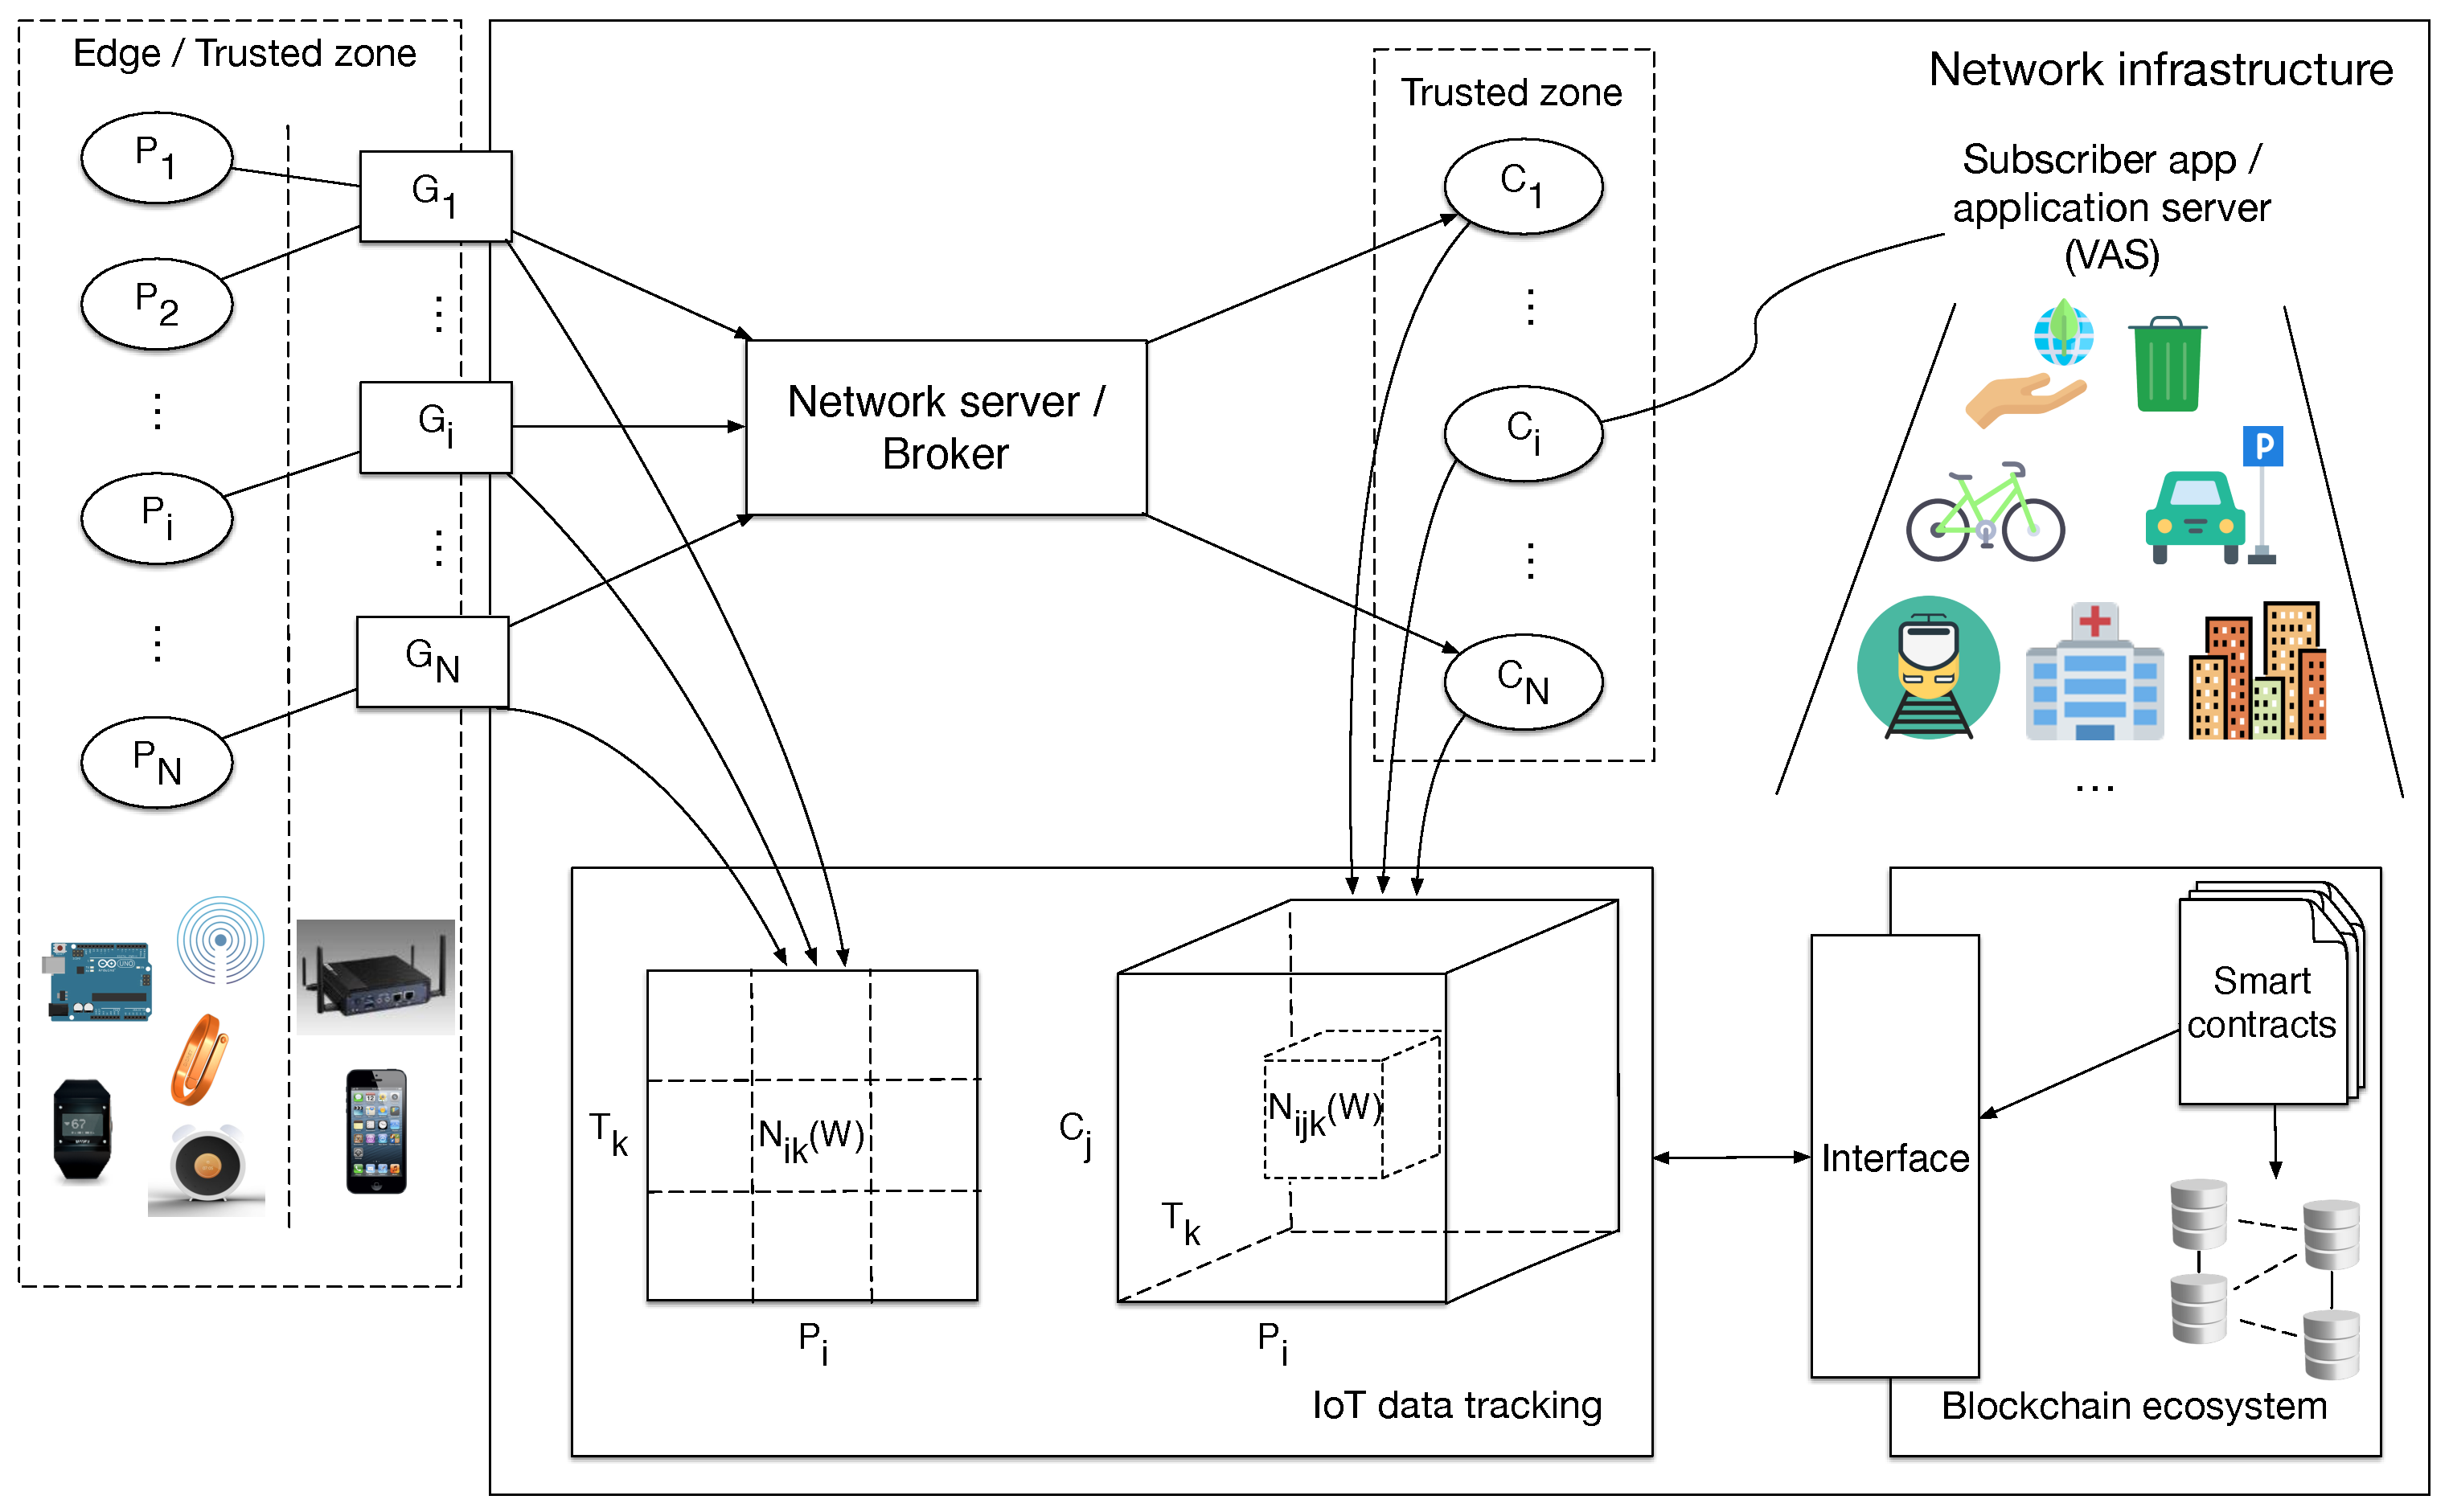
\includegraphics[width=0.6\textwidth]{figures/IoT-tracking-arch-2}
	\caption{Reference architecture for decentralised IoT data traffic metering based on blockchain and Smart Contracts}
	\label{fig:iot-tracking-arch-2}
\end{figure*}

Figure 1 concretely illustrates this setting. To remove the need for a centralised trust, we push it towards the borders of the data flow network by defining two \textit{trusted zones}.
The first trusted zone includes all the elements at the edge of the network infrastructure, such as the IoT devices $P$ and the gateways $ G_i $, whereas the second one includes $ C $.
%The latter range from monitoring, to health applications, assets tracking, smart city applications, etc.
IoT data are still routed towards the VASs through brokers--using a publish-subscribe pattern--or network servers.
However, we now assume that a new, independent IoT data tracking component receives the unilateral cubes by gateways and VASs.
%Finally, a Smart Contract deployed on a blockchain periodically accesses the traffic cubes to realize settlement services and resolve possible conflicts.
Finally, a Smart Contract, decentralised trusted service deployed on a blockchain, periodically accesses the traffic cubes to realize settlement services and resolve possible conflicts.

\subsection{Consistency and settlement with unilateral cubes}

Suppose that, at the end of $W$, every $p_i$ and $c_j$ produce  unilateral cubes relative to $W$. 
These form the set
\begin{equation}\label{eq:all-cubes}
\{ \mathit{cube}^p(W, p_i) \}_{p_i \in P}\cup \{\mathit{cube^s}(W, c_j) \}_{c_j \in C} 
\end{equation}
As each of these cubes provides a partial view of the same complete cube $ \mathit{cube}(W) $ that would have been generated centrally by a broker, we expect that the values found in these cubes be somehow consistent with $ \mathit{cube}(W) $.

The pub/sub model implies that the number of messages sent by $p_i$ with topic $t_k$ during $W$ must be equal (assuming no messages are lost and ignoring duplicate transmissions, as in MQTT QoS level 3) to the number of messages each $c_i$ that subscribes to $t_k$ receives from $p_i$. 
We can capture this constraint formally using our cubes notation, as follows.
%
For each $ p_i \in P, t_k \in T, c_j \in \mathit{sub}(t_k)$:
{\begin{equation}\label{eq:cubes-consistency}
\begin{split}
& \mathit{cube}^p(W, p_i)[t_k] = N^s_{ik}(W) = \\
& \mathit{cube}(W)[p_i, t_k, c_j]  = N_{ijk}(W) = \\
& \mathit{cube^s}(W, c_j)[p_i, t_k]
\end{split}
\end{equation}
%\vspace{-10pt}
%\begin{definition}
We say that the set (\ref{eq:all-cubes}) of all unilateral cubes is \textit{consistent} at $W$, if and only their contents satisfy constraint (\ref{eq:cubes-consistency}).
%\begin{end}
We use this definition as a basis for settlement of message exchanges within each $W$, in the general case that the broker cannot be trusted to provide a single global cube that is complete and correct.
%
Specifically, in our architecture we  now assume that a new, independent component receives all cubes in (\ref{eq:all-cubes}) at the end of each $W$, and checks their consistency using (\ref{eq:cubes-consistency}). 
In the next section we discuss a practical implementation of this idea, where this new component is realised as a Ethereum Smart Contract and unilateral cubes are posted publicly as part of blockchain transactions.

In this decentralised scenario, such a settlement service must be able to deal with two inter-dependent issues, namely (a) \textit{completeness} and (b) \textit{consistency} of the set (\ref{eq:all-cubes}) of all cubes.

The case when set (\ref{eq:all-cubes}) is both complete and consistent is straightforward and results in successful settlement, as all information for settlement is available, and there are no disagreements.

When the set of cubes is incomplete, we may try to use (\ref{eq:cubes-consistency}) to propagate missing values from the more complete to the less complete cubes. 
More precisely, suppose $ \mathit{cube}^p(W, p_i) $ is missing for a $p_i$.
If $ N_{ijk}(W) = \mathit{cube^s}(W, c_j)[p_i, t_k] $ is available for some $t_k$ and some $ c_j \in \mathit{sub}(t_k) $, then we set $  \mathit{cube}^p(W, p_i)[t_k]=  N_{ijk}(W) $.
In practice, this can be viewed as ``taking $ c_j $s word for $p_i$s missing report''.

Symmetrically, the settlement service may use the available $ \mathit{cube}^p(W, p_i)$, in combination with subscription information $ \{\mathit{sub}(t_k) | t_k \in T \}$, to fill in missing values in 
$  \mathit{cube^s}(W, c_j)  $, i.e., by setting 
$ \mathit{cube^s}(W, c_j)[p_i, t_k]  =  \mathit{cube}^p(W, p_i)[t_k]$ for each $t_k$ and each $c_j \in \mathit{sub}(t_k)$.
%
Of course, there is no guarantee that all missing values can be propagated. 
In this case, settlement for the $\langle p_i, c_j \rangle$ pairs corresponding to the missing cube entries is simply not possible.

The final, and perhaps most important case occurs when constraint (\ref{eq:cubes-consistency}) is violated for some combination of $\langle p_i, c_j, t_k \rangle$.
This may be due to the malicious cases of over-reporting producers, or under-reporting subscribers.
%
Either of these  scenarios manifests itself as inequalities in (\ref{eq:cubes-consistency}), of the form:
\begin{equation}\label{eq:inconsistencies}
\mathit{cube}^p(W, p_i)[t_k] > \mathit{cube^s}(W, c_j)[p_i, t_k]
\end{equation}
In this situation, we are able to detect the inconsistency, but we may not have enough information to determine whether $p_i$, $c_j$, or both are guilty of fraud.
Such determination is beyond the scope of this paper, but in the final discussion section we present initial ideas on promoting a self-regulating marketplace in the presence of such unresolvable inconsistencies.
%
In our initial implementation, described next, the settlement service simply reports the detected inequalities.

%%%%
%%% Andrea + Angelo
\section{Initial proof-of-concept realisation}  \label{eq:realisation}


\subsection{Background notions: Blockchain and Smart Contract}  \label{sec:blockchain}
Blockchain is essentially a distributed ledger of information (e.g., a transaction from A to B in the bitcoin world), a copy of which cannot be arbitrarily altered without being spotted and for which consistency of each information can be achieved through a decentralized and distributed consensus, without requiring trust in any third party but instead, through large and flat pool of so-called miners using cryptographic primitives~\cite{nakamoto2008bitcoin}.
Blockchain has been later leveraged to manage Smart Contracts, small pieces of software that encode a set of conditions and actions that a machine can interpret and that can be executed as expected using the blockchain infrastructure without third party involvement or supervision~\cite{Buterin2014}. Smart contracts represent therefore a well-suited decentralized tool to implement Traffic Cube and Settlement functionalities. Being one of the most adopted and well-supported by the developer community, we decide to use Ethereum Smart Contract implementation.

In the Ethereum network, any node uses a virtual machine (EVM), which can execute code of arbitrary algorithmic complexity, to execute smart contracts, the integrity of whose is always guaranteed. A smart contract can perform various state updates and account balancing.  
Executing a smart contract results in one or more transactions to be validated. Each transaction has a cost (e.g., fee) associated, which translates into incentive for any miner within the network to independently execute it. 
More specifically, any operation being performed within a transaction consumes a fixed amount of Gas. Miners fees are therefore proportional to the amount of Gas used. Gas price is measured in terms of Ether (the Ethereum cryptocurrency). Every transaction specifies the gas price a smart contract is willing to pay for its execution, thus, the total fee paid for a transaction is the result of Gas amount multiplied by the Gas selected price.

%The second element of our approach is based on the use of emergin Blockchain and Smart Contracts tecnhology.

%\note{FIXME -- still a dump of Michele's text . background}

%Blockchain is essentially a distributed ledger of information (e.g., a transaction from A to B in the bitcoin world), a copy of which cannot be arbitrarily altered without being spotted and for which consistency of each information can be achieved in a decentralized and distributed way, without requiring trust in any third party. These properties, that in the bitcoin world provides a very strong business case (e.g., removing transaction costs associated to clearinghouse functionalities when transferring money), can also provide a trust case for exchanging access to different assets, without requiring trust among parties.

%Decentralized Applications (DApps) use assets and services from different sources, not controlled by only one entity (in contrast to the traditional centralized client/server web). Using smart contracts and off-chain information makes more practical to develop new DApps. s-Health apps can be seen as a particular type of DApps. Bitcoin is the first DApp built on top of the blockchain: it is a digital and interoperable currency (i.e., it does not require conversion across the world), using the blockchain infrastructure and some complex cryptographic algorithms, to achieve (nearly) zero transaction fees while avoiding the double-spending problem (e.g., possibility to spend a given amount twice) and without requiring to trust in any third party to police this risk. Thinking about the value of different assets, bitcoin and alt-coin (i.e., bitcoin plus metadata) can provide an interoperable and open cross-domain incentives platform for redistributing the value created from assets sharing, transparently covering the interests of all the involved assets providers.

%Blockchain has been later leveraged to manage Smart Contracts, small pieces of software that encode a set of conditions and actions that a machine can interpret and that can be executed as expected using the blockchain infrastructure without third party involvement or supervision \cite{Buterin2014}. These functionalities can be interesting when it comes to give permission to access different assets (datasets and devices) only for specific purposes.

%Blockchain is usually adopted by Decentralized Autonomous Organizations (DAOs), which require neither written statements nor physical governance bodies, to run on code expressed by a set of Smart Contracts. This concept is interesting for organizations where different stakeholders can vote and agree on the rules for sharing their assets, e.g., for particular social benefits or research purpose, thus deciding how their rewards should be distributed while influencing and supporting the creation of specific s-Health services. Through DAOs, the principles, rules and benefits deriving from data sharing can be distributedly enforced without requiring any trusted third party. While this is a powerful concept to achieve autonomy and avoid misuse, particular attention is required in order to properly encode the right human assisted governance structure in the DAOs. This might require a governance body that supervises the rules implemented as DAO by an open developers community, following a rigorous, open, transparent and accounted review process.


%\note{ANDREA}


%\authornote{We need reference to ETH architecture, with APIs call and a snippet of the code. We can add some numbers on how much this will cost to run and consequently set up a minimum cost for each data in order to keep infrastructure sustainable.
%Logic: “data” is a “count cube”. The platform generates a stream of these cubes at a certain rate, which is tunable using the window size on the TrackerDB. The arrival rate of the cubes determines the frequency at which contracts are executed, and therefore the cost over time.
%}
\subsection{Implementation}
The generation of unilateral cubes can rely on different implementation choices made within the Data Producers (DP) and VAS Trusted Zones. This does not affect the properties of the Traffic Cube and Settlement, because liability is pushed at the edge. Section X provides some detail on how unilateral cube generation can be implemented. 
Here we instead focus on detailed implementation of the Traffic Cube and Settlement functionalities using smart contracts. 
We developed them using Solidity, the Ethereum's scripting language. To implement the contracts we assigned an Ethereum account to each DP and VAS. We connected these accounts to our private Ethereum test network, deployed on a single node with 6-core Intel Xeon E5-2640 and 16GB of RAM. We wrote, deployed and evaluated smart contracts in the network by using the Ethereum web browser based IDE REMIX, connected to our private chain through RPC protocol. In our implementation, accounts prepare and send the transactions to the blockchain to instances of Geth through RPC. To measure gas consumption, we used the debug tool provided by Remix and we observed the difference in the account balance before and after invoking the contract to measure the transaction cost.

A limitation of Ethereum smart contracts is that they cannot directly access off-chain data about real-world state and events. In our case this represents a challenge in acquiring unilateral cubes value. More precisely, smart contracts are independently executed by any node in the chain, thus, each execution needs to retrieve such information from an off-chain source independently, without any assurance of the information integrity.
To overcome this limit, the concept of \emph{oracle} has been introduced. Simply speaking, an oracle is a special contract that serves data requests from traditional contracts, by sourcing them from designated data feeds. 
Two options are possible for implementing oracles. The first one is relying on existing proxy services. Oraclize provides a \emph{programmable} oracle that can interact with any datasource selected among a predefined set of standard channels. In addition Oraclize provides an authenticity proof by means of a TLSNotary proof[cite] which guarantees the authenticity and integrity of the retrieved data. These functionalities come at a cost. For each off-chain query, Oraclize requires a fee which includes a commission, ranging from 0.01\$ to 0.04\$, and a refund of the Gas used to perform the transaction. 
The other option is when each party of the contract, Data Producer and VAS, independently update their unilateral cubes by pulling their values from cubes generator located within their Trusted Zones and then creating a transaction which embeds the cubes in the blockchain. This way any node executing the smart contract will have the same copy of that cube. As a result, costs associated to the use of an external oracle service, such as Oraclize, can be saved. Because in our model responsibility and liability of producing faulty cubes is placed to Data Producers and VASs, this option well suffices to our needs.
Figure XX shows pseudo-code of our settlement contract. For the sake of simplicity, this snippet of code only accounts for the single Data Producer and the single VAS scenario, although generalization are straightforward.
The contract first requests the involved parties to provide their unilateral cubes; then it uses this information to perform the actual settlement, by combining the two unilateral cubes. If the processed combined cube is consistent then a payment to the producer is performed, otherwise, a dispute resolution mechanism should be invoked.

\begin{algorithm}
	\caption{Cube settlement contract pseudo-code}\label{settlement_contract}
\begin{algorithmic}
	\IF{sender $\neq$ authorizedAddress}
	\STATE throw
	\IF{queryId $=$ producerQuery}
	\STATE producer $\gets$ unilateralCube
	\STATE vasQuery $\gets$ update()
	\ELSIF{queryId $=$ vasQuery}
	\STATE vas $\gets$ unilateralCube
	\IF {producer $=$ vas}
	\STATE transfer(producerAccount, dataPrice, result)
	\ELSE
	\STATE disputeResolution()
	\ENDIF
	\ENDIF
	\ENDIF
\end{algorithmic}
\end{algorithm}

When a dispute resolution is invoked, payments are retained from being performed due to impossibility to clearly identify the correct unilateral cube. However a reputation mechanism can be implemented in order to penalize both parties involved in a given settlement transaction and to ultimately promote honest behaviour. As it is not expected that reputation computation will require off-chain interaction~\cite{schaub2016trustless,carboni2015feedback}, we are confident that while not considering its implementation in this phase this will not significantly affect the overall contract execution costs.

\section{Evaluation and Lessons learnt}  \label{sec:evaluaton}

Aim of this section is to quantify the cost of the smart contract described above and the associated cube settlement operations. By considering the scenario in which one VAS consumes the data of one Data Producer, we evaluate how the cost of performing such contract changes depending on the number of data exchanged and the number of settlements transactions required. Considering different quantity of exchanged data reflect the different purpose of the exchange (event-based data rather than real-time series acquisition). Nevertheless the reason for considering a variation in the number of required settlement needs some clarification. The most natural strategy will be to perform the settlement at the end of each contractually agreed data exchange, however in the early stage of an hypothetical market place where new producers and VASs join without necessarily trusting each other nor having an already established reputation, two situations might occur:
\begin{itemize}
	\item {Data producers and VASs have low reputation hence their trust level is low and the risk of claiming wrong unilateral cubes high. In this case, by performing more than one cube settlement, in an initial rump-up phase of a given data exchange will allow them to mutually increase their reputation and trust;}
	\item {Data producers and VASs have already high reputation hence they are expected to act honestly. In this case cube settlements may occur with a lower rate, eventually only at the end of a data exchange phase, because the risk of producing faulty cubes is mitigated.}
\end{itemize}
%1- 
%2- 

By evaluating the cost of performing the settlement operations we are able to define the minimum price that VASs should pay for each consumed data in order to sustain the settlement infrastructure and eventually generate profit for the Data Producers.

We define the minimum data price as the amount of Ether needed to at least cover the cost of contract deployment and transactions for performing cubes settlement operations. This means that if a producer sells data at the minimum price, its profit will be zero. 
At the time of writing one Ether costs 220\$, however, its price is still very volatile\footnote{https://etherscan.io/chart/etherprice}.

As result, transaction cost may frequently vary, thus leading to uncertainty about the economic feasibility of a specific application. We analysed the capability of Ethereum to support a stable transaction cost by tuning the Gas price. The main drawback when setting a low gas price is the increase of time required before a transaction is validated. Assuming a range of gas price between 0.9 Gwei and 20 Gwei (0.0000000009 and 0.00000002 Ether respectively), as minimum and average reported by the Ethereum network in 2017, the time required for a transaction to be validated in the chain varies from 2 minutes to 14 seconds\footnote{https://etherscan.io/chart}. As explained before, even in the case of multiple settlements, we don’t expect that meaningful data exchange will last less than 2 minutes, thus we consider a viable choice to select the current minimum Gas price.


Figure~\ref{fig:overall} shows a general overview of the minimum data price by varying the frequency of cubes clearance operations and the amount of transferred data. The price is directly proportional to the increase of the number of cubes settlement performed while inversely proportional to the increase of data amount exchanged. Clearly, the more the data a VAS purchases, the less impacts the cost of performing cubes settlement. Depending on the type of data exchanged and trustworthiness of involved parties using this figure clearly shows how an optimal settlement strategy can always be found to dynamically adapt the number of settlement operations.

\begin{figure*}[t]
	\centering
	\subfigure[Overall cost]{
		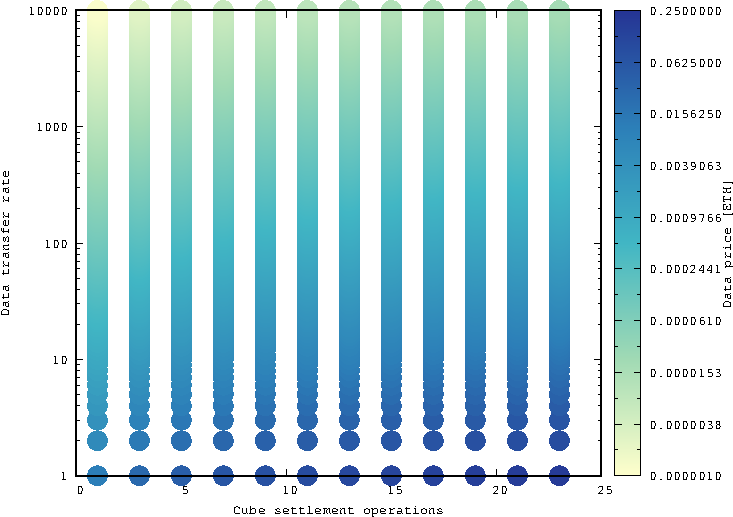
\includegraphics[width=.31\textwidth]{figures/feeNew-crop}
		\label{fig:overall}
	}%
	\subfigure[without Oraclize]{
		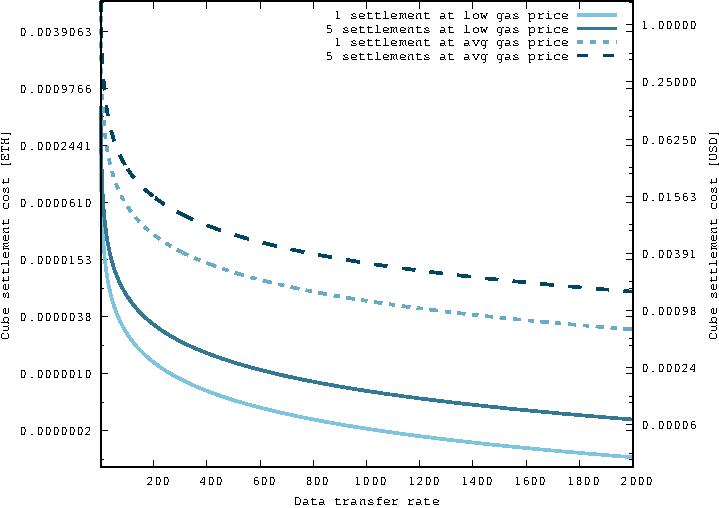
\includegraphics[width=.31\textwidth]{figures/resultSimple2-crop}
		\label{fig:noOraclize}
	}%
	\subfigure[with Oraclize]{
		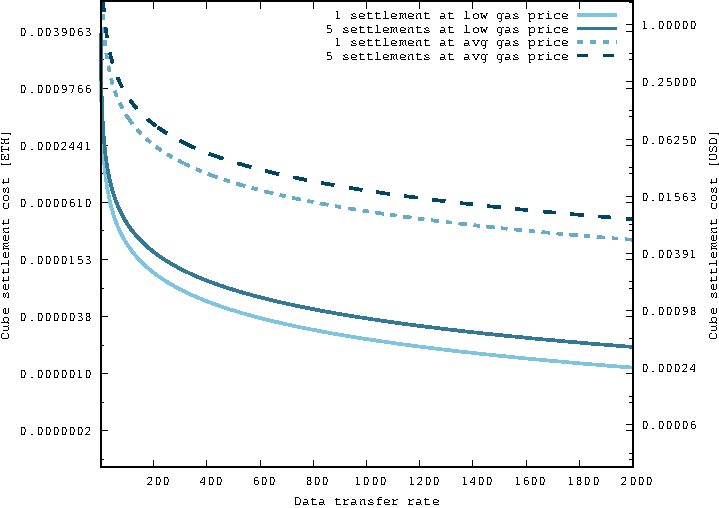
\includegraphics[width=.31\textwidth]{figures/resultOraclize2-crop}
		\label{fig:withOraclize}
	}%
	\caption{Cost of performing cube settlement operations for different data transfer rate.}
	\label{fig:all}
\end{figure*}

Figures~\ref{fig:noOraclize} and~\ref{fig:withOraclize} show the total cost of performing 1 or 5 cubes settlement operations for a fixed amount of transferred data, when considering a gas price ranging from 0.9 Gwei to 20 Gwei.
More specifically, figure~\ref{fig:noOraclize} shows the case when each party of the contract use its oracle implementation, while figure~\ref{fig:withOraclize} shows the case when Oraclize functionalities are used. 
It worth noticing the large costs increase (on average 4 times more), due to the commission and refund of the Gas used to perform the transaction to be paid to Oraclize. 
Without Oraclize, the cost of a single cube settlement transaction ranges from 0.000099 Ether to 0.0022 Ether when the gas price selected is 0.9 Gwei and 20 Gwei respectively. The more amount of data is transferred, the less impact the transaction cost has per single data. In fact, when performing a cube settlement operation spread over 2000 data, its cost ranges from 0.00000012 Ether to 0.0000028 Ether. Alternatively, when performing 5 cube settlement over 2000 data, their cost ranges from 0.0000003 Ether to 0.000007 Ether.
%1.26e-07	3.15e-07	2.8e-06	7e-06
When using Oraclize, the cost of a single cube settlement transaction ranges from 0.00036 Ether to 0.008 Ether when the gas price selected is 0.9 Gwei and 20 Gwei respectively. When performing a cube settlement operation spread over 2000 data, its cost ranges from 0.0.0000011 Ether to 0.0.000024 Ether. Alternatively, when performing 5 cube settlement over the same amount of data, their cost ranges from 0.0000018 Ether to 0.00004 Ether.
%\note{Add oraclize graph description}
%1.1081205e-06	1.8299205e-06	2.46249e-05	4.06649e-05

In order to derive a profitable data price, we can consider two examples: 1) an air quality monitoring application running on a Low Power Wide Area Network (LPWAN), such as Lora, that generates data every hour, resulting in 24 measurements per day; 2) a heart rate monitoring application (e.g., fitbit), with sampling frequency of 1 second, 1 minute.  
Assuming that the cost of performing settlement operations has to be equal to 2\% of the price for that data amount.and that only one cube settlement is performed per day, Table X shows that data price ranges from 0.000001\$ to 0.00028\$ depending on the gas price selected. 
Table XXX shows estimated data price for different use cases, such as a heart rate monitoring application (e.g., fitbit), with sampling frequency of 1 second, 1 minute and 1 hour.   



%\authornote{
%\note{new from Michele}
%
%	\begin{itemize}
%\item test assuming no need of settlement, value are the same
%\item Test different time periods for cube generation, fine grained vs to larger interval, up to daily
%\item Invariance wrt to period for cube computation 
%\item Dependency wrt to number of sources and VAS (not addressed here)
%	\end{itemize}
%}
%
%
%\authornote{
%\note{old list}
%	\begin{itemize}
%		\item Are smart contracts an adequate implementation model to realise a fair marketplace?
%\item Are there limitations in the reconciliation phase?
%\item Cost of operating and marketplace: executing transactions and how to control them -- contract activated in an adaptive mode.  Who owns the contracts?  (ideal answer: nobody. Participants share the cost of transactions)
%\item Scalability: how the cubes decouple the data flow rates from the transaction frequency
%\item Data marketplace model is preliminary and not validated on real world use cases. It is based on minimal data semantics (ie the topic) and has no notion of more sophisticated contract models.
%	\end{itemize}
%}
%
%
%\authornote{
%\note{lessons learnt}
%
%	\begin{itemize}
%\item event vs time series, costs and requirements
%\item Liability of oracolize model for trust; requirements of new interfaces
%\item Volatility of market and price
%	\end{itemize}
%}

%%%%

\section{Conclusion and future work}
Our initial work encourages us to further develop the idea of a decentralised data marketplace, where benefits such as interoperability, transparency and fairness are achievable and cost affordable. However we recognised that the cube settlement component is a very important but still only one building block of such an infrastructure, in which existing less-critical centralised and new decentralised elements will have to be combined. In future we plan to experiment and test the effectiveness of the reputation based reconciliation strategy and to develop the complete architecture for a trusted and transparent data marketplace. This will include Data Producers and VASs discovery service, contract creation and discovery platform and the definition of an open governance model associated to it, promoting public and open creation and review of settlement contracts (extending the github model (\url{github.com}).



% conference papers do not normally have an appendix


% use section* for acknowledgment
%\section*{Acknowledgment}


%The authors would like to thank...

%\bibliographystyle{IEEEtran}
%\bibliography{IEEEabrv,iot-conf}

\small %\footnotesize
\input{iot-conf-static.bbl}

% trigger a \newpage just before the given reference
% number - used to balance the columns on the last page
% adjust value as needed - may need to be readjusted if
% the document is modified later
%\IEEEtriggeratref{8}
% The "triggered" command can be changed if desired:
%\IEEEtriggercmd{\enlargethispage{-5in}}

% references section

% can use a bibliography generated by BibTeX as a .bbl file
% BibTeX documentation can be easily obtained at:
% http://mirror.ctan.org/biblio/bibtex/contrib/doc/
% The IEEEtran BibTeX style support page is at:
% http://www.michaelshell.org/tex/ieeetran/bibtex/
%\bibliographystyle{IEEEtran}
% argument is your BibTeX string definitions and bibliography database(s)
%\bibliography{IEEEabrv,../bib/paper}
%
% <OR> manually copy in the resultant .bbl file
% set second argument of \begin to the number of references
% (used to reserve space for the reference number labels box)




% that's all folks
\end{document}


